\documentclass[border=6pt]{standalone}
\usepackage{amsmath,amssymb}
\usepackage{tikz}
\usetikzlibrary{arrows.meta,shadows,calc,backgrounds}
\begin{document}
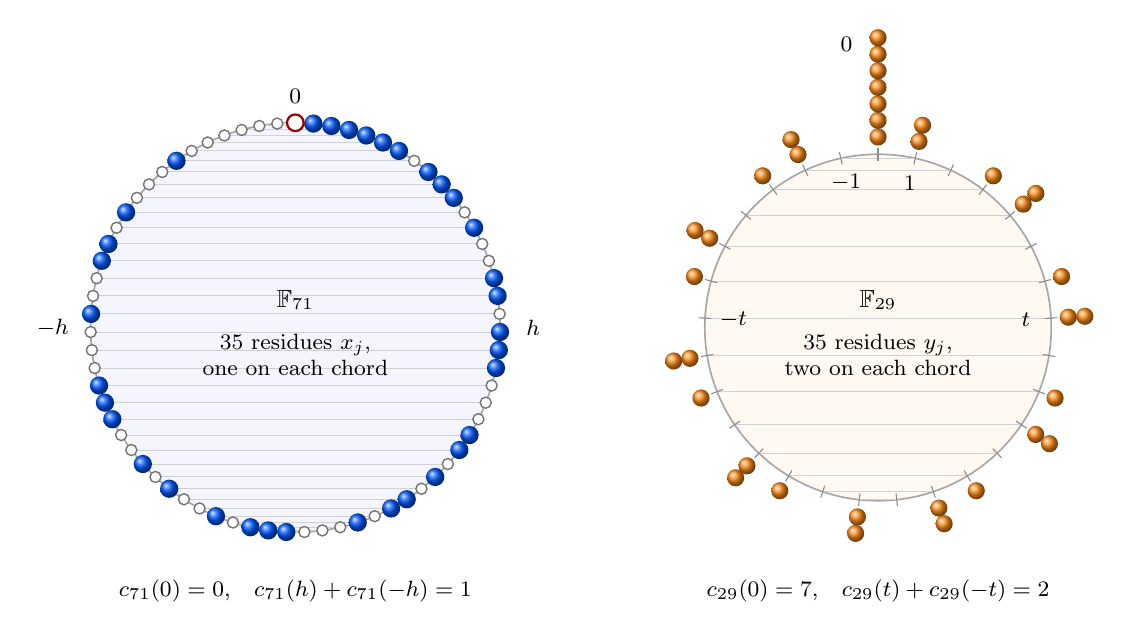
\begin{tikzpicture}[
  lab/.style={font=\footnotesize},
  tick/.style={line width=0.4pt,black!45},
  chord/.style={line width=0.35pt,black!18},
  hollow/.style={circle,inner sep=0pt,minimum size=4pt,draw=black!55,line width=0.5pt,fill=white}]
% ------------------------------------------------------------ F_71
\def\R{2.6}
\begin{scope}[on background layer]
  \fill[blue!4] (0,0) circle (\R);
  \draw[black!35,line width=0.6pt] (0,0) circle (\R);
  \foreach \h in {1,...,35} { \draw[chord] ({90-(360/71)*\h}:\R) -- ({90+(360/71)*\h}:\R); }
\end{scope}
\foreach \h in {0,...,70} { \draw[tick] ({90-(360/71)*\h}:{\R-0.07}) -- ({90-(360/71)*\h}:{\R+0.07}); }
\foreach \h in {1,...,70} { \node[hollow] at ({90-(360/71)*\h}:\R) {}; }
\foreach \h in {1,2,3,4,5,6,8,9,10,12,15,16,18,19,20,24,25,27,29,30,32,36,37,38,40,43,45,48,49,50,54,57,58,60,64}
  { \shade[ball color=blue!65!cyan] ({90-(360/71)*\h}:\R) circle (3.3pt); }
\node[hollow,minimum size=6pt,draw=red!60!black,line width=0.8pt] at (90:\R) {};
\node[lab,anchor=south] at (90:{\R+0.12}) {$0$};
\node[lab] at (0:{\R+0.42}) {$h$};
\node[lab] at (180:{\R+0.48}) {$-h$};
\node[font=\small] at (0,0.35) {$\mathbb F_{71}$};
\node[lab,align=center] at (0,-0.35) {$35$ residues $x_j$,\\ one on each chord};
\node[lab,align=center] at (0,-\R-0.75) {$c_{71}(0)=0$,\quad $c_{71}(h)+c_{71}(-h)=1$};
% ------------------------------------------------------------ F_29, case (c)
\begin{scope}[shift={(7.4,0)}]
\def\R{2.2}
\begin{scope}[on background layer]
  \fill[orange!5] (0,0) circle (\R);
  \draw[black!35,line width=0.6pt] (0,0) circle (\R);
  \foreach \t in {1,...,14} { \draw[chord] ({90-(360/29)*\t}:\R) -- ({90+(360/29)*\t}:\R); }
\end{scope}
\foreach \t in {0,...,28} { \draw[tick] ({90-(360/29)*\t}:{\R-0.08}) -- ({90-(360/29)*\t}:{\R+0.08}); }
% seven residues at 0
\foreach \k in {0,...,6} { \shade[ball color=orange!90] (90:{\R+0.22+0.21*\k}) circle (3.1pt); }
% two residues on each pair {t,-t}: pattern 1+1, 2+0, 0+2
\foreach \t in {1,...,14} {
  \pgfmathtruncatemacro{\m}{mod(\t,3)}
  \ifcase\m
    \shade[ball color=orange!90] ({90-(360/29)*\t}:{\R+0.22}) circle (3.1pt);
    \shade[ball color=orange!90] ({90+(360/29)*\t}:{\R+0.22}) circle (3.1pt);
  \or
    \shade[ball color=orange!90] ({90-(360/29)*\t}:{\R+0.22}) circle (3.1pt);
    \shade[ball color=orange!90] ({90-(360/29)*\t}:{\R+0.43}) circle (3.1pt);
  \or
    \shade[ball color=orange!90] ({90+(360/29)*\t}:{\R+0.22}) circle (3.1pt);
    \shade[ball color=orange!90] ({90+(360/29)*\t}:{\R+0.43}) circle (3.1pt);
  \fi
}
\node[lab,anchor=east] at ($(90:{\R+1.4})+(-0.2,0)$) {$0$};
\node[lab] at ({90-(360/29)}:{\R-0.32}) {$1$};
\node[lab] at ({90+(360/29)}:{\R-0.32}) {$-1$};
\node[lab] at ({90-(360/29)*7}:{\R-0.32}) {$t$};
\node[lab] at ({90+(360/29)*7}:{\R-0.36}) {$-t$};
\node[font=\small] at (0,0.35) {$\mathbb F_{29}$};
\node[lab,align=center] at (0,-0.35) {$35$ residues $y_j$,\\ two on each chord};
\node[lab,align=center] at (0,-\R-1.15) {$c_{29}(0)=7$,\quad $c_{29}(t)+c_{29}(-t)=2$};
\end{scope}
\end{tikzpicture}
\end{document}
